\chapter{Further Work}

\section{Verilog Preprocessor}

\subsection{Additional Customisation}
\begin{enumerate}
  \item LFSR with variable width
  \item variable number of inputs/outputs to DUT
\end{enumerate}

\subsection{Unified Interface}
\begin{enumerate}
  \item Qsys
  \item Quartus
  \item Software
\end{enumerate}


\section{Automatic Delay Reconfiguration}

Since finding out the delay of the DUT is useful for further simplifying the configuration process of the framework, a delay tester is built within the driver.
It counts the number of cycles for the DUT to produce its output as \texttt{dut\_delay}, but it still has a few limitations in its design.
As such, using this to reconfigure the driver to monitor delay on the fly is not yet possible.
How this might be achieved will be discussed in the Further Work chapter of this report.

The delay tester is built with a simple FSM.

\begin{figure}[H]
  \centering
  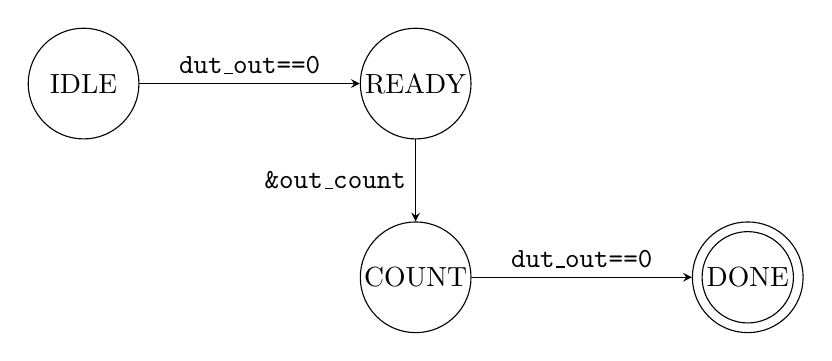
\begin{tikzpicture}
  [
    x=1em, y=1em,
    node/.style =
      {draw, circle, align=center, inner sep=0pt, minimum size=4em},
    sarrow/.style =
      { ->, >=stealth, font=\ttfamily}
  ]
  \node [node] at ( 0, 7)  (i) {IDLE};
  \node [node] at (12, 7) (r) {READY};
  \node [node] at (12, 0)  (c) {COUNT};
  \node [node] at (24, 0)  (d) {DONE};
  \node [draw, circle, inner sep=0pt, minimum size=3.3em] at (24, 0)  (dd) {};

  \draw [sarrow] (i.east)  -- node[above] {dut\_out==0}  (r.west);
  \draw [sarrow] (r.south) -- node[left]  {\&out\_count} (c.north);
  \draw [sarrow] (c.east)  -- node[above] {dut\_out==0}  (d.west);
\end{tikzpicture}
  \caption{Delay Tester FSM}
  \label{DelayTesterFSM}
\end{figure}

We first start a counter called \texttt{out\_count}.
Whenever this reaches all 1's, the driver output is set to some value with a known safe DUT output.
In this example, the safe output value is 0, which means when the delay tester is active, no other output from the driver can result in a DUT output of 0.

\begin{figure}[H]
  \centering
  \input{illu/delay_tester}
  \caption{3-bit Delay Tester Waveform}
  \label{DelayTesterWF}
\end{figure}

The FSM starts in state IDLE.
When the first 0 output is detected from the DUT, the FSM enters the READY state.
It now knows that it can enter the COUNT state when the \texttt{out\_count} becomes all 1's again, triggering the next safe test input.
The FSM leaves the COUNT state for the DONE state when the safe output of 0 is detected.
The delay tester process is now complete and \texttt{out\_count} can be deactivated.

With this, the DUT's delay in clock cycles is the same as the number of cycles that the FSM stayed in state COUNT.
The delay counter \texttt{delay\_out} increments itself every cycle if the FSM is in that state.
When the FSM enters the DONE state, we the value of the delay counter is the delay of the DUT.
With a 3-bit counter as shown in the timing diagram, it can measure this delay for up to 8 clock cycles.
Longer delays can be measured by extending the width of \texttt{out\_count}.


without:
394.01MHz
with delay tester:
Fmax, Restricted Fmax
374.25, 315.06
slow 1100mV 85C

\subsection{Reference Delay}
Currently reference is sub-monitor -> which needs to pass through dut\_out as well.
To have a pure module, need this delay control.